\documentclass[11pt,a4paper]{article}
% LaTeX source of the report, laid out like the Natural Language Engineering template.
% The official nle.sty is not used (it is not freely available); the layout is reproduced with
% standard packages. Compile with: pdflatex report.tex (twice). Works on Overleaf.
\usepackage[T1]{fontenc}
\usepackage[utf8]{inputenc}
\usepackage{lmodern}
\usepackage[a4paper,left=33mm,right=33mm,top=30mm,bottom=30mm]{geometry}
\usepackage{graphicx}
\usepackage{fancyhdr}
\usepackage{titlesec}
\usepackage{array}
\usepackage{caption}
\usepackage{booktabs}
\usepackage{microtype}
\usepackage[hidelinks]{hyperref}
\captionsetup[table]{labelsep=period,font=small,justification=centering,position=top}
\captionsetup[figure]{labelsep=period,font=small,justification=centering,name=Fig.}
\titleformat{\section}[block]{\centering\bfseries\large}{\thesection}{1em}{}
\titleformat{\subsection}[block]{\centering\bfseries\itshape}{\thesubsection}{1em}{}
\titleformat{name=\section,numberless}[block]{\centering\bfseries\large}{}{0pt}{}
\titlespacing*{\section}{0pt}{2.5ex plus 1ex}{1.5ex}
\titlespacing*{\subsection}{0pt}{2ex plus 1ex}{1ex}
\setlength{\parindent}{1.5em}
\setlength{\parskip}{0pt}
\newcommand{\shorttitle}{Hinglish to English machine translation}
\newcommand{\shortauthor}{S. Kumari and others}
\pagestyle{fancy}
\fancyhf{}
\renewcommand{\headrulewidth}{0pt}
\fancyhead[CO]{\small\itshape\shorttitle}
\fancyhead[RO]{\small\thepage}
\fancyhead[LE]{\small\thepage}
\fancyhead[CE]{\small\itshape\shortauthor}
\fancypagestyle{plain}{\fancyhf{}\renewcommand{\headrulewidth}{0pt}%
  \fancyhead[L]{\small\itshape Natural Language Engineering \upshape 1 (1): 1--11. Course project submission}%
  \fancyhead[R]{\small\thepage}}
\begin{document}
\thispagestyle{plain}
\begin{center}
{\LARGE\itshape Translating code-mixed Hinglish into English: how much does pretraining help when data is scarce?\par}
\vspace{1.2em}
{\large\textsc{Swati Kumari, Pinky Rana, Vinay Kumar and Ujjval Baijal}\par}
\vspace{0.4em}
{\small\itshape Group 8 (P08), Deep Learning course project, Sitare University, India\par}
\vspace{0.8em}
{\itshape ( Received 22 November 2026 )\par}
\end{center}
\vspace{0.4em}\hrule\vspace{0.8em}
\begin{center}\textbf{Abstract}\end{center}\vspace{-0.4em}
{\small Hinglish, Hindi written in the Latin alphabet and mixed with English, is common on social media but hard to translate because parallel data is scarce, spelling is not fixed and English words appear unchanged. We ask how much pretraining helps for translating Hinglish into English compared with training from scratch. On the PHINC corpus we fix a cleaned train/validation/test split, fixing junk translations, cut tweets and HTML codes found in the raw data, and compare four systems under one evaluation protocol: an LSTM with Bahdanau attention and a Transformer, both trained from scratch, and mBART-50 and mT5-small, both zero-shot and fine-tuned. Fine-tuned mBART-50 is best (36.76 BLEU, 57.87 chrF), followed by the Transformer trained from scratch (28.51 BLEU), fine-tuned mT5-small (18.97) and the LSTM (8.97). Pretraining therefore helped clearly for a model built for translation, but not for every pretrained model. A hand-tagged analysis of the worst translations shows different failure modes for each system, and noisy references account for a large share of them. All results are single runs on one corpus.\par}
\vspace{0.8em}\hrule\vspace{0.4em}

\section{Introduction}
Social media users in India routinely write Hindi in the Latin alphabet and mix it with English inside a single sentence, for example \textit{kya baat hai bhaiya} (``wow, brother''). This style, called Hinglish, is a form of code-mixing. It is hard for machine translation for three reasons: parallel data is scarce, Hindi words in Roman script have no fixed spelling (\textit{kya}, \textit{kyaa}, \textit{kyaaa}), and many English words appear unchanged between the two languages, so a model has to decide for every word whether to translate it or to copy it.

Large pretrained multilingual models are the usual answer to scarce data, but they were not trained on Roman-script Hindi as a language of its own, and it is not clear how much they help compared with a smaller model trained from scratch on the little data that exists. This is the question of this project: \textbf{how much does pretraining help on a low-resource, code-mixed translation task compared with training from scratch?}

We study it on the PHINC corpus (Srivastava and Singh 2020) with four systems that use one fixed data split and one scoring function: a recurrent LSTM with Bahdanau attention (Bahdanau et al. 2015) and a Transformer (Vaswani et al. 2017), both trained from scratch, and the pretrained mBART-50 (Tang et al. 2020) and mT5-small (Xue et al. 2021), each evaluated zero-shot and after fine-tuning. Our contributions are:

\begin{itemize}\setlength\itemsep{0pt}
\item a cleaned, fixed train/validation/test split of PHINC, with the data problems we found in the raw file documented and fixed;
\item a shared evaluation protocol (BLEU and chrF through one function) so that all systems are comparable;
\item results for six system configurations on 1,345 test sentences, with a hand-tagged error analysis of the 50 worst translations of each trained system;
\item an open, tested code base with continuous integration, from which every number in this report can be regenerated.
\end{itemize}
The rest of the paper is organised as follows. Section 2 gives background, Section 3 describes the data, Section 4 the systems and the evaluation, Section 5 the results, Section 6 the error analysis, and Sections 7 and 8 discuss limitations and conclude.

\section{Background and related work}
\textbf{Code-mixed translation.} Code-mixed text is noisy and low-resource, and parallel corpora for it are small. PHINC (Srivastava and Singh 2020) is a parallel corpus of Hinglish social media sentences with English translations written by human annotators; it is the data used here.

\textbf{Neural translation from scratch.} Sequence-to-sequence models with attention (Bahdanau et al. 2015), built on LSTM networks (Hochreiter and Schmidhuber 1997), learn to align target words with source words. The Transformer (Vaswani et al. 2017) replaces recurrence by self-attention and is the standard architecture today. Subword vocabularies such as byte-pair encoding (Sennrich et al. 2016), trained with SentencePiece (Kudo and Richardson 2018), let a model represent rare and misspelled words as sequences of known pieces.

\textbf{Pretrained multilingual models.} mBART (Liu et al. 2020) is pretrained by denoising text in many languages and, as mBART-50 (Tang et al. 2020), fine-tuned for translation between 50 languages. mT5 (Xue et al. 2021) is a multilingual text-to-text model pretrained on web text. IndicTrans2 (Gala et al. 2023) is a translation model for Indian languages that is a natural candidate for Hindi; we prepared code for it but did not run it (Section 7).

\textbf{Evaluation.} We report BLEU (Papineni et al. 2002) and chrF (Popovi\'c 2015), computed with sacreBLEU (Post 2018). BLEU compares word n-grams with the reference and is known to be harsh on short and noisy sentences; chrF compares character n-grams and is more forgiving of spelling variation, which suits Hinglish.

\section{Data}
\subsection{The PHINC corpus}
PHINC contains 13,738 rows, each a Roman-script Hinglish sentence taken from social media and its English translation. We lowercase all text and replace URLs by the token \texttt{\textless{}url\textgreater{}}; mentions, hashtags and emoticons are kept because the English reference keeps them too.

\subsection{Problems in the raw file}
Reviews of our own pipeline found problems in the raw data that would have distorted every result, and we fixed them before any final training:

\begin{itemize}\setlength\itemsep{0pt}
\item \textbf{Junk translations.} 234 rows have an English side that is only an emoticon such as \texttt{)}, \texttt{\$} or \texttt{-)}. A model trained on them learned to output \texttt{)}. Rows with no letter on either side are dropped.
\item \textbf{Cut tweets.} 51 pairs come from tweets that were cut at the HTML code \texttt{\&amp;}, so source and reference are two halves of one English sentence (for example \texttt{...from h\&} and \texttt{m tomorrow}). Pairs where a side ends with a bare \texttt{\&} are dropped.
\item \textbf{HTML codes.} \texttt{\&amp;} and \texttt{\&lt;} are decoded.
\item \textbf{Duplicates.} Exact duplicate (Hinglish, English) pairs are removed, so no identical pair is in two splits.
\end{itemize}
\subsection{Fixed split}
After cleaning, the data is shuffled with seed 42 and cut into 80\% training, 10\% validation and 10\% test data (Table~\ref{tab:data}). All systems are trained on the training split, tuned on the validation split and evaluated once on the test split. Vocabularies and tokenizers are built from the training split only. About 28\% of the Hinglish words also appear unchanged in the English sentence, which shows how much English is mixed in. The same Hinglish sentence can still occur with a different translation in two splits (one validation and one test sentence also occur in training).

The references are noisy. 10 of the 1,345 test references (0.74\%) contain no real word at all, only emoticons, mentions, hashtags or \texttt{\textless{}url\textgreater{}} (for example \texttt{) \textless{}url\textgreater{}}). We left them in so that all systems are scored on the same fixed split.

\begin{table}[t]
\caption{\textit{Statistics of the fixed split (words per sentence, after cleaning)}}\label{tab:data}
\centering\small
\begin{tabular}{lrrrrr}
\hline\hline
\textbf{Split} & \textbf{Pairs} & \textbf{Hinglish mean} & \textbf{Hinglish max} & \textbf{English mean} & \textbf{English max} \\
\hline
Train & 10,762 & 13\textperiodcentered{}3 & 40 & 12\textperiodcentered{}5 & 46 \\
Validation & 1,345 & 13\textperiodcentered{}1 & 37 & 12\textperiodcentered{}5 & 37 \\
Test & 1,345 & 13\textperiodcentered{}1 & 37 & 12\textperiodcentered{}2 & 37 \\
\hline\hline
\end{tabular}
\end{table}
\section{Systems and evaluation}
\subsection{LSTM with Bahdanau attention}
The first system is a recurrent encoder-decoder. A bidirectional LSTM reads the Hinglish sentence; an LSTM decoder produces the English sentence one word at a time and, at every step, attends over all source positions with additive (Bahdanau) attention. It uses word-level vocabularies of the words seen at least twice in the training data, embeddings of size 256, a decoder of size 512, dropout 0.3, the Adam optimiser (Kingma and Ba 2015) with learning rate 0.001, label smoothing (Szegedy et al. 2016) of 0.1 and early stopping on validation loss. Training stopped after 15 epochs. About 12\% of the English training words are rare and become the unknown token \texttt{\textless{}unk\textgreater{}}; the model therefore learned to output \texttt{\textless{}unk\textgreater{}}, and blocking it during decoding raised BLEU from 6.50 to 8.97. We decode with beam search of size 5.

\begin{figure}[t]\centering
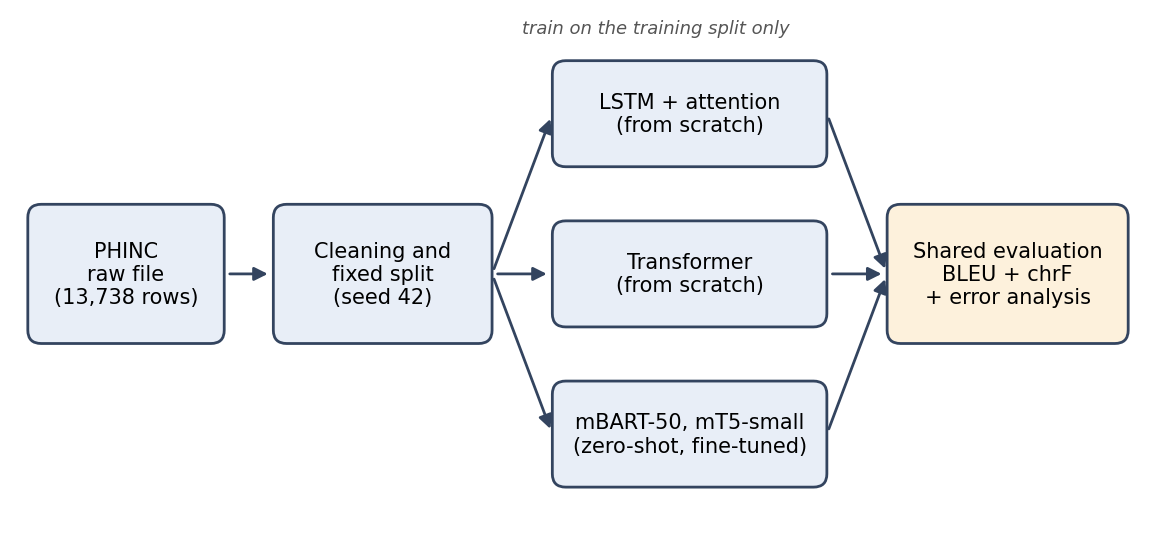
\includegraphics[width=0.98\textwidth]{figures/pipeline.png}
\caption{Overview of the experimental pipeline. All systems read the same split and are scored by the same evaluation function.}\label{fig:pipeline}
\end{figure}
\subsection{Transformer trained from scratch}
The second system is a Transformer encoder-decoder (Vaswani et al. 2017) trained from random initialisation. It is built from PyTorch (Paszke et al. 2019) encoder and decoder layers; the sinusoidal positional encoding, the causal and padding masks, a single embedding shared by the source input, the target input and the output layer, and greedy and beam-search decoding are our own code. Because Hinglish spelling varies, it uses one joint SentencePiece BPE vocabulary of 4,000 pieces for both languages, trained on the training split. The vocabulary is small because the data is small: a larger one would leave many pieces with few examples. We trained two settings with d\_model 256, 4 attention heads, feed-forward size 1,024, dropout 0.3, label smoothing 0.1 and the warmup learning-rate schedule of the original paper: a 3-layer model (6.6M parameters) and a 6-layer model (12.1M parameters), for up to 40 epochs on a CPU. The 6-layer model is reported as the main result.

\subsection{Pretrained models, zero-shot and fine-tuned}
The third family uses pretrained translation models. mBART-50 (\texttt{facebook/mbart-large-50-many-to-many-mmt}) is given the Hindi source-language tag and English as target. mT5-small (\texttt{google/mt5-small}) receives the prefix ``translate Hinglish to English:''. For both we report the zero-shot score (no training) and the score after fine-tuning on the training split (mBART-50 for 3 epochs, mT5-small for 5 epochs), with learning rate 3e-5, batch size 8 with 4 gradient-accumulation steps, and beam search of size 4, on a Colab T4 GPU through the Hugging Face library (Wolf et al. 2020). The Roman-script input is passed to the tokenizers unchanged.

\subsection{Evaluation protocol}
All systems are scored by one function. It lowercases predictions and references and computes corpus BLEU and chrF with sacreBLEU. Lowercasing is necessary because the references are lowercased by our preprocessing while the pretrained models write capitalised English; without it they would be penalised only for casing. After a system is trained, its 100 lowest-scoring test translations (by sentence chrF) are saved, and 50 of them are tagged by hand with an error category for the error analysis.

\begin{table}[t]
\caption{\textit{Main settings of the trained and fine-tuned systems}}\label{tab:settings}
\centering
\begin{tabular}{>{\raggedright\arraybackslash\scriptsize}p{0.16\textwidth}>{\raggedright\arraybackslash\scriptsize}p{0.21\textwidth}>{\raggedright\arraybackslash\scriptsize}p{0.23\textwidth}>{\raggedright\arraybackslash\scriptsize}p{0.17\textwidth}>{\raggedright\arraybackslash\scriptsize}p{0.17\textwidth}}
\hline\hline
\textbf{Setting} & \textbf{LSTM + attention} & \textbf{Transformer (6 layers)} & \textbf{mBART-50} & \textbf{mT5-small} \\
\hline
Vocabulary & words seen at least 2 times & joint BPE, 4,000 pieces & pretrained subwords & pretrained subwords \\
Size & embedding 256, encoder 2x256, decoder 512 & d\_model 256, 4 heads, feed-forward 1,024, 6+6 layers & pretrained, large & pretrained, small \\
Dropout / label smoothing & 0.3 / 0.1 & 0.3 / 0.1 & model default / none & model default / none \\
Optimiser, learning rate & Adam, 0.001 & Adam, warmup 1600 steps & AdamW, 3e-5 & AdamW, 3e-5 \\
Batch size & 64 & 64 & 8 \ensuremath{\times} 4 accumulation & 8 \ensuremath{\times} 4 accumulation \\
Epochs & up to 30, early stopping (stopped at 15) & up to 40 (no early stop) & 3 & 5 \\
Beam size & 5 & 5 & 4 & 4 \\
Seed & 42 & 42 & 42 & 42 \\
\hline\hline
\end{tabular}
\end{table}
\section{Results}
Table~\ref{tab:results} and Figure~\ref{fig:comparison} show the test scores of all systems on the 1,345 test sentences. The fine-tuned mBART-50 is clearly best (36.76 BLEU, 57.87 chrF). The Transformer trained from scratch is second (28.51 BLEU), and it is above the zero-shot mBART-50 (22.14). Fine-tuned mT5-small (18.97) and the LSTM (8.97) follow, and zero-shot mT5-small is useless (0.01 BLEU).

\begin{table}[t]
\caption{\textit{Test results (1,345 sentences); higher is better}}\label{tab:results}
\centering\small
\begin{tabular}{rllrr}
\hline\hline
\textbf{Rank} & \textbf{System} & \textbf{Training} & \textbf{BLEU} & \textbf{chrF} \\
\hline
1 & mBART-50 fine-tuned & pretrained + fine-tuned & 36\textperiodcentered{}76 & 57\textperiodcentered{}87 \\
2 & Transformer, 6 layers & from scratch & 28\textperiodcentered{}51 & 50\textperiodcentered{}32 \\
3 & mBART-50 zero-shot & pretrained, no training & 22\textperiodcentered{}14 & 38\textperiodcentered{}35 \\
4 & mT5-small fine-tuned & pretrained + fine-tuned & 18\textperiodcentered{}97 & 33\textperiodcentered{}79 \\
5 & LSTM + attention & from scratch & 8\textperiodcentered{}97 & 27\textperiodcentered{}71 \\
6 & mT5-small zero-shot & pretrained, no training & 0\textperiodcentered{}01 & 2\textperiodcentered{}33 \\
\hline\hline
\end{tabular}
\end{table}
\begin{figure}[t]\centering
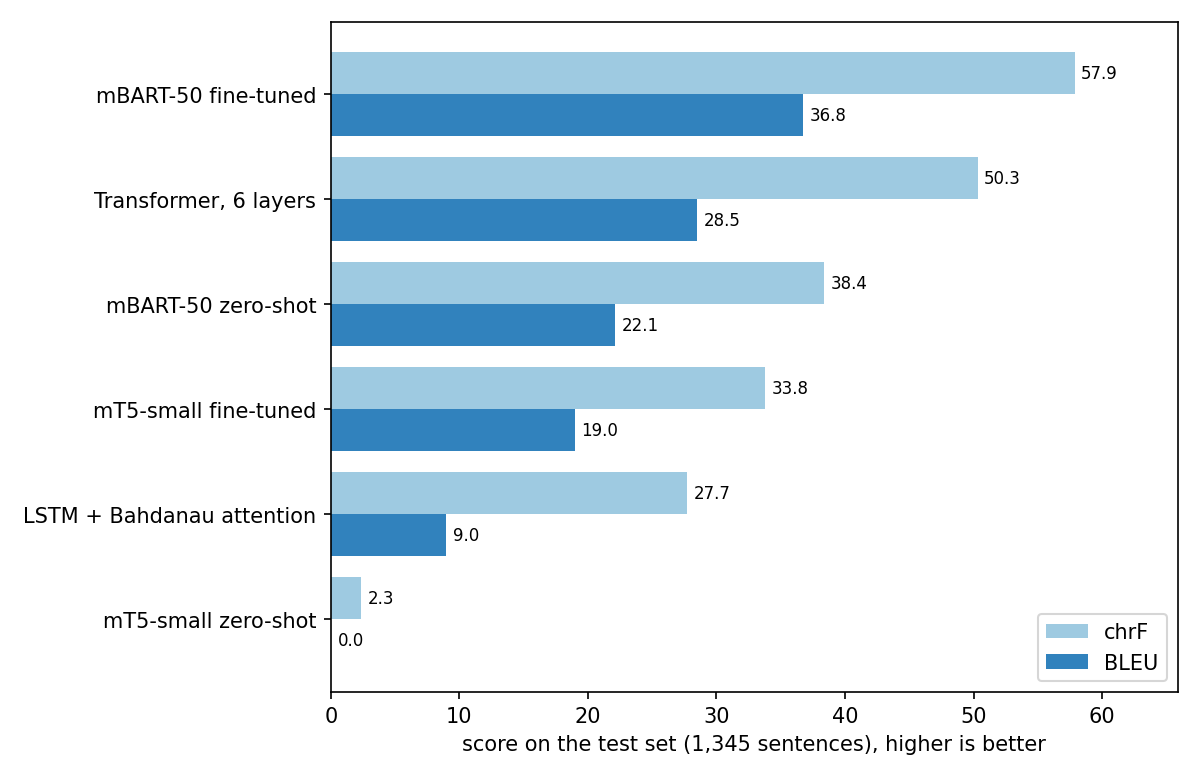
\includegraphics[width=0.85\textwidth]{figures/comparison.png}
\caption{BLEU and chrF of all systems on the test set.}\label{fig:comparison}
\end{figure}
\subsection{Effect of decoding and model size}
Beam search improved over greedy decoding for both systems we trained from scratch (Table~\ref{tab:decoding}): by 1.33 BLEU for the LSTM and 1.60 for the 6-layer Transformer. The 3-layer Transformer (28.43 BLEU, 49.77 chrF) is practically as good as the 6-layer one (28.51 BLEU, 50.32 chrF): the BLEU difference of 0.08 is within the noise of a single run, and the deeper model needed about twice the training time. Neither Transformer run stopped early; the validation loss was still falling slowly at epoch 40, so longer training might give a little more.

\begin{table}[t]
\caption{\textit{Greedy decoding against beam search (test BLEU)}}\label{tab:decoding}
\centering\small
\begin{tabular}{lrrr}
\hline\hline
\textbf{System} & \textbf{Greedy} & \textbf{Beam search} & \textbf{Gain} \\
\hline
LSTM + attention (beam 5) & 7\textperiodcentered{}64 & 8\textperiodcentered{}97 & 1\textperiodcentered{}33 \\
Transformer, 3 layers (beam 5) & 27\textperiodcentered{}78 & 28\textperiodcentered{}43 & 0\textperiodcentered{}65 \\
Transformer, 6 layers (beam 5) & 26\textperiodcentered{}91 & 28\textperiodcentered{}51 & 1\textperiodcentered{}60 \\
\hline\hline
\end{tabular}
\end{table}
\begin{figure}[t]\centering
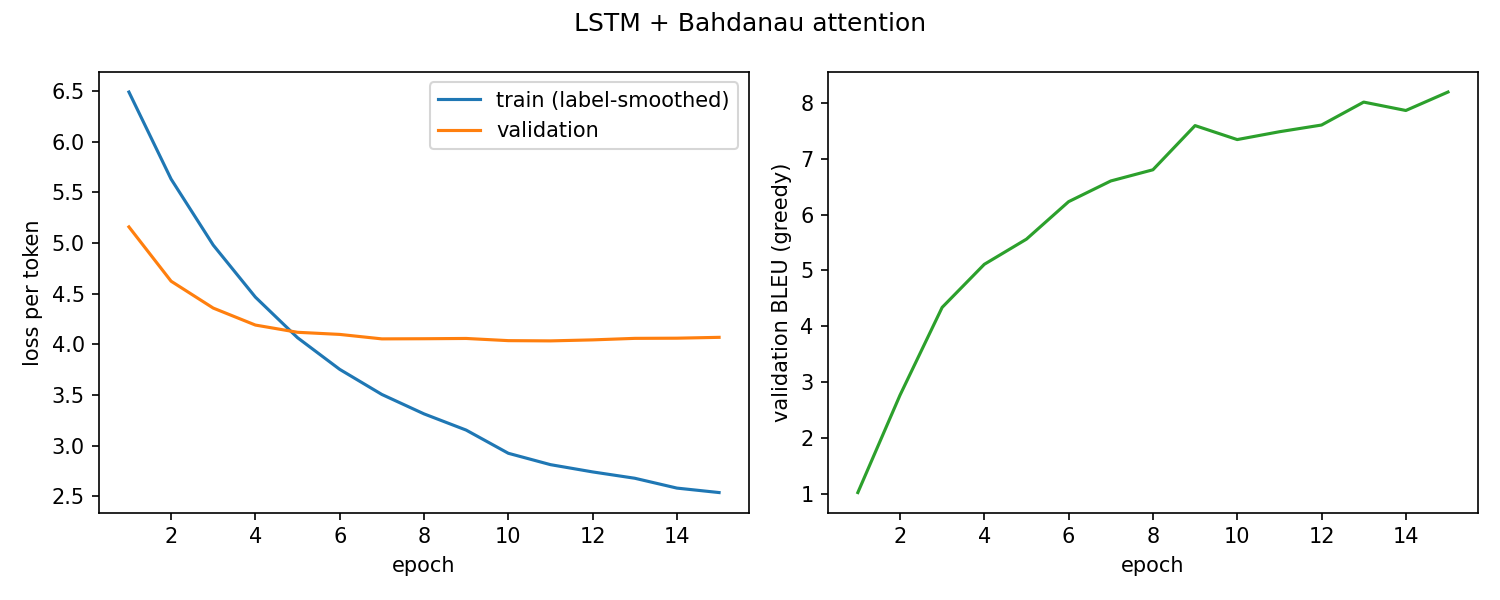
\includegraphics[width=0.98\textwidth]{figures/lstm_curves.png}
\caption{Training curves of the LSTM: the training loss keeps falling while the validation loss stays flat after about epoch 5 (left), and the validation BLEU rises slowly (right).}\label{fig:curves}
\end{figure}
\section{Error analysis}
For each trained system, the 50 worst test translations (lowest sentence chrF) were tagged by hand with an error category. The categories were chosen by the person tagging each system, so the columns of Table~\ref{tab:errors} are only roughly comparable, and the table describes the worst sentences, not all errors. Table~\ref{tab:examples} shows real examples.

\begin{table}[t]
\caption{\textit{Hand-tagged error categories among the 50 worst test translations of each system}}\label{tab:errors}
\centering\small
\begin{tabular}{lrrrr}
\hline\hline
\textbf{Error category} & \textbf{LSTM} & \textbf{Transformer} & \textbf{mT5-small} & \textbf{mBART-50} \\
\hline
Wrong meaning & 17 & 20 &  & 21 \\
Noisy reference & 9 & 13 & 3 & 14 \\
Dropped words & 2 & 1 & 24 & 1 \\
Junk output & 14 & 2 & 10 &  \\
Repetition & 4 & 1 & 13 & 1 \\
Hindi word left untranslated &  & 11 &  &  \\
Wrong word choice & 1 & 1 &  & 5 \\
Transliteration error &  &  &  & 5 \\
English not copied & 3 &  &  &  \\
Code-mixing issue &  &  &  & 3 \\
Correct but worded differently &  & 1 &  &  \\
\textbf{Tagged rows} & \textbf{50} & \textbf{50} & \textbf{50} & \textbf{50} \\
\hline\hline
\end{tabular}
\end{table}
\noindent What the table shows:

\begin{itemize}\setlength\itemsep{0pt}
\item \textbf{mBART-50} writes fluent English. Its worst cases are mostly a wrong meaning for a colloquial phrase, or a noisy reference.
\item \textbf{mT5-small} mostly drops words or repeats itself, often producing only a mention or a few characters.
\item \textbf{The Transformer} almost never produces junk output, but when it does not know a Hindi word it often copies it into the English, because both languages share one BPE vocabulary.
\item \textbf{The LSTM} produces junk such as \texttt{) :p} in 14 of its 50 worst cases, which its author traced to emoticon-only training references.
\item \textbf{Noisy references} are among the worst cases of every system (3 to 14 of 50). For example, the reference of \texttt{rt @sheikhimaan : news flash : iss baar bheja tha . jeet gaye .} is only \texttt{) \textless{}url\textgreater{}}.
\end{itemize}
\begin{table}[t]
\caption{\textit{Examples of tagged errors (real rows from the error files)}}\label{tab:examples}
\centering
\begin{tabular}{>{\raggedright\arraybackslash\scriptsize}p{0.22\textwidth}>{\raggedright\arraybackslash\scriptsize}p{0.19\textwidth}>{\raggedright\arraybackslash\scriptsize}p{0.14\textwidth}>{\raggedright\arraybackslash\scriptsize}p{0.22\textwidth}>{\raggedright\arraybackslash\scriptsize}p{0.18\textwidth}}
\hline\hline
\textbf{Hinglish input} & \textbf{Reference} & \textbf{System} & \textbf{System output} & \textbf{Category} \\
\hline
\texttt{mobarak ied mobarak ??} & \texttt{happy eid.} & Transformer & \texttt{mobarak ied mobarak ??} & Hindi word left untranslated \\
\texttt{mobarak ied mobarak ??} & \texttt{happy eid.} & mBART-50 & \texttt{mobarak ied mobarak ??} & Transliteration error \\
\texttt{kya yr maine b mis kr diya \#uhh} & \texttt{damn man, even i missed it} & mT5-small & \texttt{@uhhhhhhhhhhh} & Repetition \\
\texttt{hamari bus main bhi ek dengu aata tha ,} & \texttt{in our bus also one dengu used to come ,} & LSTM & \texttt{) :p} & Junk output \\
\texttt{haha kya haal chaal hai?} & \texttt{haha, what is going on?} & mBART-50 & \texttt{haha what's the matter?} & Wrong word choice \\
\hline\hline
\end{tabular}
\end{table}
\section{Discussion and limitations}
\subsection{Does pretraining help?}
For mBART-50, yes. Fine-tuned mBART-50 is 8.25 BLEU above the best system trained from scratch, and fine-tuning added 14.62 BLEU over its zero-shot score. Even zero-shot, mBART-50 (22.14) is 13.17 BLEU above the LSTM. For mT5-small the answer is no: zero-shot it is useless, and after fine-tuning (18.97) it stays 9.54 BLEU below the Transformer trained from scratch. Likely reasons are that mT5-small is a small general-purpose model that was not pretrained for translation, and that we fine-tuned it with a learning rate of 3e-5, lower than the 3e-4 that is commonly used for mT5, so it may be under-tuned. We did not test this. The honest summary is that a pretrained model built for translation helps a lot, while a small general-purpose model does not necessarily.

\subsection{A Transformer from scratch is competitive}
With only about 10.8 thousand training pairs, the Transformer reached 28.51 BLEU, above zero-shot mBART-50. The BPE vocabulary is probably a large part of the reason: the LSTM, with word-level vocabularies, loses many rare words to \texttt{\textless{}unk\textgreater{}}. The 19.5 BLEU gap between the LSTM and the Transformer is therefore a mixture of architecture and tokenisation; we did not train an LSTM with BPE to separate the two.

\subsection{Limitations}
\begin{itemize}\setlength\itemsep{0pt}
\item \textbf{Single runs.} Every system was trained once with seed 42. Differences of a few tenths of BLEU, such as the 0.08 BLEU between the two Transformers, are not meaningful. We computed no confidence intervals or significance tests, because only the 100 worst predictions of each system were saved, not all test predictions.
\item \textbf{Noisy references.} PHINC translations are sometimes wrong or loosely aligned, which lowers all scores. Removing the emoticon-only test references would change the split again, so we kept them.
\item \textbf{Not done.} IndicTrans2 and a Roman-to-Devanagari transliteration experiment were prepared but not run; mT5 was not tuned; we did not train on smaller fractions of the data to see where pretraining helps most, and we did not break the scores down by sentence length or amount of code-mixing.
\item \textbf{Different taggers.} The errors of each system were tagged by a different person with their own categories.
\item \textbf{One dataset.} All data is social media text from one corpus; the results may not carry over to other kinds of Hinglish.
\end{itemize}
\section{Conclusion}
On PHINC, a pretrained translation model fine-tuned on our small training set (mBART-50, 36.76 BLEU) is clearly better than a Transformer trained from scratch (28.51 BLEU), which is in turn far better than an LSTM with attention (8.97 BLEU). The result does not extend to every pretrained model, since fine-tuned mT5-small (18.97 BLEU) is below the from-scratch Transformer. The most useful lessons of the project concerned data and evaluation: cleaning junk translations, cut tweets and HTML codes from the raw file, and scoring all systems in exactly the same way, changed which conclusions we could trust. Future work is to run IndicTrans2, to tune mT5, to repeat the runs with several seeds and test significance, and to measure where pretraining helps most by training on growing fractions of the data.

\section*{Author contributions}
\begin{table}[t]
\caption{\textit{Contributions of the authors}}\label{tab:contrib}
\centering
\begin{tabular}{>{\raggedright\arraybackslash\scriptsize}p{0.22\textwidth}>{\raggedright\arraybackslash\scriptsize}p{0.76\textwidth}}
\hline\hline
\textbf{Author} & \textbf{Contribution} \\
\hline
Swati Kumari & Repository, data pipeline (download, cleaning, fixed split, vocabulary helper), shared BLEU/chrF evaluation, tests and continuous integration, comparison script, README and this report. \\
Pinky Rana & LSTM with Bahdanau attention, its results and error analysis; code reviews that found the lowercasing bug, the junk translations and the cut tweets in the data. \\
Vinay Kumar & Fine-tuning code for mBART-50, mT5 and IndicTrans2, the Colab notebook, and the fine-tuned and zero-shot results and error analysis for mBART-50 and mT5. \\
Ujjval Baijal & Transformer trained from scratch, the comparison of two model sizes, its results and error analysis. \\
\hline\hline
\end{tabular}
\end{table}
\section*{Code and data availability}
The code, the result files and the continuous-integration setup are in the project repository (github.com/Swati89923/Translate-Roman-script-code-mixed-Hinglish-into-English). PHINC is publicly available from Zenodo (doi:10.5281/zenodo.3605597); data files and model checkpoints are not committed. Running \texttt{python src/compare.py} regenerates the ranking, the chart and the error tables from the result files.

\section*{References}
\begin{list}{}{\leftmargin=1.5em\itemindent=-1.5em\itemsep=2pt\parsep=0pt}
\small
\item Bahdanau, D., Cho, K. and Bengio, Y. (2015) Neural machine translation by jointly learning to align and translate. \textit{Proceedings of the 3rd International Conference on Learning Representations (ICLR)}.
\item Gala, J. \textit{et al.} (2023) IndicTrans2: towards high-quality and accessible machine translation models for all 22 scheduled Indian languages. \textit{Transactions on Machine Learning Research}.
\item Hochreiter, S. and Schmidhuber, J. (1997) Long short-term memory. \textit{Neural Computation} \textbf{9}(8): 1735--1780.
\item Kingma, D. P. and Ba, J. (2015) Adam: a method for stochastic optimization. \textit{Proceedings of the 3rd International Conference on Learning Representations (ICLR)}.
\item Kudo, T. and Richardson, J. (2018) SentencePiece: a simple and language independent subword tokenizer and detokenizer for neural text processing. \textit{Proceedings of EMNLP 2018: System Demonstrations}, pp. 66--71.
\item Liu, Y., Gu, J., Goyal, N., Li, X., Edunov, S., Ghazvininejad, M., Lewis, M. and Zettlemoyer, L. (2020) Multilingual denoising pre-training for neural machine translation. \textit{Transactions of the Association for Computational Linguistics} \textbf{8}: 726--742.
\item Papineni, K., Roukos, S., Ward, T. and Zhu, W.-J. (2002) BLEU: a method for automatic evaluation of machine translation. \textit{Proceedings of the 40th Annual Meeting of the Association for Computational Linguistics (ACL)}, pp. 311--318.
\item Paszke, A. \textit{et al.} (2019) PyTorch: an imperative style, high-performance deep learning library. \textit{Advances in Neural Information Processing Systems 32 (NeurIPS)}.
\item Popovi\'c, M. (2015) chrF: character n-gram F-score for automatic MT evaluation. \textit{Proceedings of the Tenth Workshop on Statistical Machine Translation}, pp. 392--395.
\item Post, M. (2018) A call for clarity in reporting BLEU scores. \textit{Proceedings of the Third Conference on Machine Translation: Research Papers}, pp. 186--191.
\item Sennrich, R., Haddow, B. and Birch, A. (2016) Neural machine translation of rare words with subword units. \textit{Proceedings of the 54th Annual Meeting of the Association for Computational Linguistics (ACL)}, pp. 1715--1725.
\item Srivastava, V. and Singh, M. (2020) PHINC: a parallel Hinglish social media code-mixed corpus for machine translation. \textit{Proceedings of the Sixth Workshop on Noisy User-generated Text (W-NUT 2020)}.
\item Szegedy, C., Vanhoucke, V., Ioffe, S., Shlens, J. and Wojna, Z. (2016) Rethinking the Inception architecture for computer vision. \textit{Proceedings of the IEEE Conference on Computer Vision and Pattern Recognition (CVPR)}, pp. 2818--2826.
\item Tang, Y., Tran, C., Li, X., Chen, P.-J., Goyal, N., Chaudhary, V., Gu, J. and Fan, A. (2020) Multilingual translation with extensible multilingual pretraining and finetuning. \textit{arXiv preprint} arXiv:2008.00401.
\item Vaswani, A., Shazeer, N., Parmar, N., Uszkoreit, J., Jones, L., Gomez, A. N., Kaiser, L. and Polosukhin, I. (2017) Attention is all you need. \textit{Advances in Neural Information Processing Systems 30 (NeurIPS)}.
\item Wolf, T. \textit{et al.} (2020) Transformers: state-of-the-art natural language processing. \textit{Proceedings of EMNLP 2020: System Demonstrations}.
\item Xue, L., Constant, N., Roberts, A., Kale, M., Al-Rfou, R., Siddhant, A., Barua, A. and Raffel, C. (2021) mT5: a massively multilingual pre-trained text-to-text transformer. \textit{Proceedings of the 2021 Conference of the North American Chapter of the Association for Computational Linguistics (NAACL-HLT)}.
\end{list}
\end{document}
